\documentclass{article}

\usepackage{tabularx}

% https://tex.stackexchange.com/a/129100/125609, to draw the pico ampremeter
\usepackage{tikz}
\usetikzlibrary{arrows}
\usetikzlibrary{shapes}
\newcommand*\circled[1]{\tikz[baseline=(char.base)]{
		            \node[shape=circle,draw,inner sep=1pt] (char) {#1};}}

% NOTE: To put equations in their environment we need either `float` or
% `caption`.  We use float to put equations and other environments exactly
% where they appear in the code with the `H` placeholder, and for that we
% redefine the `equ` environment sort of twice, so this is a bit flaky but
% it works.
\usepackage{caption}
\usepackage{subcaption}

\DeclareCaptionType{equ}[][]
\captionsetup[equ]{name=נוסחא}
\usepackage{float}
\floatstyle{plain}
% https://www.overleaf.com/learn/latex/Positioning_of_Figures
\newfloat{equ}{H}{eq}[section]
\floatname{equ}{נוסחא}

\DeclareCaptionType{graph}[][]
\captionsetup[graph]{name=גרף }

% to includegraphics
\usepackage{graphicx}

% to fix itemize lists:
% https://tex.stackexchange.com/a/53453/125609
\usepackage{enumitem}
\setlist[itemize,1]{label={\fontfamily{cmr}\fontencoding{T1}\selectfont\textbullet}}

% To crop inserted images: https://tex.stackexchange.com/questions/57418/crop-an-inserted-image
\usepackage[export]{adjustbox}

% Links
\usepackage{hyperref}
\hypersetup{colorlinks = true,
	citecolor = gray,
	linkcolor = red,
	citecolor = green,
	filecolor = magenta,
	urlcolor = cyan
}

\usepackage[version=4]{mhchem}

% To include plots by matplotlib
\usepackage{pgf}
\usepackage{pgfplots}
\pgfplotsset{compat=newest}
% Note we use resizebox as explained here through out the document https://tex.stackexchange.com/a/582956/125609

\usepackage{geometry}
 \geometry{
 a4paper,
 top=30mm,
 left = 25mm,
 right = 25mm,
 bottom=30mm,
 headheight=2cm,
 headsep=2cm,
 footskip=1.5cm
}

% Language
\usepackage{polyglossia}
\setdefaultlanguage{hebrew}
\setotherlanguage{english}
\usepackage{hebrewcal}

\usepackage[
backend=biber,
isbn=false,
style=numeric,
doi = false,
sorting=ynt
]{biblatex}
% Seems to be a recommended package but it makes quotes in bibliography at the
% end appear with a question mark instead of `"`.
%\usepackage{csquotes}
\addbibresource{references.bib} % Imports bibliography file

% Fonts
\setmainfont{David CLM}
\setsansfont{Libertinus Serif}
\setmonofont{FreeMono}
\newfontfamily\hebrewfont{David CLM}[Script=Hebrew]
\newfontfamily\hebrewfontsf{Libertinus Serif}[Script=Hebrew]
\newfontfamily\hebrewfonttt{FreeMono}[Script=Hebrew]

\title{

} 
\author{
שרה לחצר ודורון בכר \\
הפקולטה לפיזיקה, טכניון - מכון טכנולוגי לישראל.
}
\date{\today}

\begin{document}
\maketitle

\begin{abstract}



\end{abstract}

\section{מבוא}
\subsection{מדידת קבוע סליל בשיטת ESR}
בניסוי זה השתמשנו בשיטת סחריר האלקטרון, שיטה בה חוקרים תכונות של חומרים בעלי אלקטרונים לא מזווגים.
בתהודת סחריר האלקטרון 
,\textenglish{ESR},
נמדדת בליעת אנרגיה של אלקטרונים בנוכחות שדה מגנטי חיצוני. השדה המגנטי גורם לאלקטרונים להסתדר במקביל ובאנטי מקביל ביחס אליו כתלות במומנטים המגנטיים שלהם. כתוצאה מכך, נוצר פיצול ברמות האנרגיה.
בעזרת אפקט זימן נוכל לקבוע כי הפרשי האנרגיות עבור אלקטרונים לא מזווגים חופשיים נתונים על פי נוסחא
\ref{equ:U_gap}.

\begin{equ}
$$ \Delta U = g \mu _B H$$
\caption{
פער אנרגטי בין רמות האנרגיה שנוצרו משדה מגנטי חיצוני-
$H$,
המגנטון של בוהר-
$\mu _B$,
וקבוע הפיצול
$g$.
}
\label{equ:U_gap}
\end{equ}
פילוג האלקטרונים בשתי רמות האנרגיה יהיה בהתאם להתפלגות בולצמן, כך שהרמה האנרגטית הנמוכה תהיה מאוכלסת יותר מהרמה האנרגית הגבוהה .

% TODO: read about stimulated emission and explain why there is an equal probability for transitions, maybe explain with fermi golden rule why most of the transitions will be from - to +.
לפיכך, בהכנסת פוטונים בעלי אנרגיה 
$\Delta U$
, יעברו יותר אלקטרונים מהרמה התחתונה לעליונה מאשר להיפך, כך שתבלע אנרגיה במערכת.

\subsection{מדידת זמן רלקסציה $T_2$}
רלקסציה היא החזרה לשיווי משקל של המגנטיזציה לאחר ערעורה, היא מאופיינת ע"י גודל הנקרא זמן רלקסציה.
קיימים שני סוגים של זמני רלקסציה:
$spin-lattice - T_1$-
ו-
$spin-spin - T_2$.
זמן הרלקסציה ספין ספין מושפע מחוסר הומוגניות של השדה המגנטי ומאינטרקציות ספין ספין הגורמות לחוסר סנכרון בפאזות הספינים.
 
ניתן לחלץ את ערכו של זמן הרלקסיה - 
$T_2$,
מתוך נוסחא
\label{equ:absorptionRate},
בעזרת רוחב הלורנציאן.


\begin{equ}
$$ P(\omega) = \frac{\omega \gamma M_z T_2 H_1^2}{1+ (\omega_0 -\omega)^2 T^2_2} $$
\caption{
קצב בליעת האנרגיה כתלות ב
$M_z$
מגנטציית הדגם,
$T_2$
זמן רלקסציה,
$\gamma = \frac{g \mu_B}{\hbar}$
ותדירות התהודה של המערכת}

\label{equ:absorptionRate}
\end{equ}
\section{מערכת הניסוי}



מערכת הניסוי מורכבת מסליל חיצוני וסליל פנימי בהם מוצב הדגם, כפי שמוצג באיור 
\ref{fig:experiment_scheme}. 
הזרם הזורם בסליל החיצוני יוצר את השדה המגנטי הגורם לפיצול רמות האנרגיה, ואילו הסליל הפנימי מספק אנרגיה למערכת הגורמת לערור האלקטרונים. 

\begin{figure}[ht!]
    \centering
    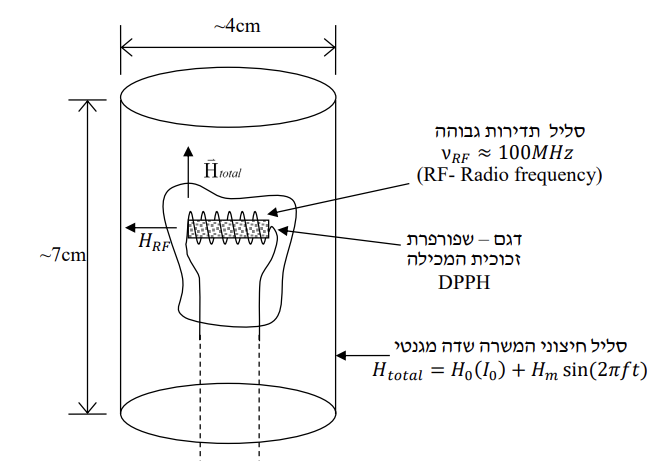
\includegraphics[width=0.7\textwidth]{schematic_setup.png}
    \caption{סכמה של מערכת הניסוי}
    \label{fig:experiment_scheme}
\end{figure}


בניגוד למקובל בספקטרוסקופיה בה משנים האנרגיה המסופקת למערכת לערעור האלקטרונים, בניסוי זה נשנה את השדה המגנטי החיצוני וכך את רמות האנרגיה.

בסליל החיצוני נזרים זרם חילופין באמפליטודה
$I_m$,
בכדי ליצור פיצול ברמות האנרגיה המשתנה בזמן שיגרום לתהודה באופן מחזורי.
בנוסף נזרים זרם ישר
$I_0$,
כך השדה המגנטי הכולל מוצג בנוסחא
\ref{equ:H_outer_inductor}.
% TODO: add the formula for the theoretical magnetic field
\begin{equ}
$$ H_{total} = k \cdot (I_0 + I_m sin(2 \pi ft))$$
\caption{
השדה המגנטי בסליל החיצוני כתלות בזרמי הסליל וקבוע הפרופורציה 
$k$.
}
\label{equ:H_outer_inductor}
\end{equ}

בסליל הקטן מוזרם זרם חילופין היוצר שדה אלקטרומגנטי 
$H_{RF}$
בתדירות קבועה
$v_{RF} \approx 100 MHz$.

לבסוף הדגם המוצב במערכת הוא פחמימן מוצק -
\textenglish{DPPH},
המכיל רדיקלים חופשיים בעלי אלקטרונים בלתי מזווגים.
הצימוד בין אלקטרונים אלה לבין הסריג האטומי הוא חלש, ולכן ערכו של
$g$
קרוב לאלקטרון חופשי ושווה ל-
$g = 2.0036 \pm 0.0002$.


מדידת בליעת האנרגיה נעשית בהסתמך כי בעת בליעה מתרחש שינוי הפרמאביליות של הדגם ומשום שהוא משמש כליבה של סליל במעגל
$LC$
קרוב לרזוננס נוכל למדוד את האפקט.

\end{document}